%% Research Background

%% A Theory section should extend, not repeat, the background to the article already dealt with in the Introduction and lay the foundation for further work. In contrast, a Calculation section represents a practical development from a theoretical basis.

%A theoretical framework is a foundational review of existing theories that serves as a roadmap for developing the arguments you will use in your own work.

%=============================================================================
%Outline.
%1. Introduction
%2. The importance of facade in a building.
%3. A brief analysis of architecture styles and the
%3. A reflexion into digital fabrication techniques specially parametric design.
%4. The principle od data driven design.
%5. An analysis into mixed reality and the advantages of introducing this  into the design review.
%=============================================================================

%///////////////////////////////////////////////////////////////
%% refined outline of theory framework

%6. **Human-Centric Design Philosophy:** Explore the historical evolution of architectural philosophies that prioritize human experience and well-being. Discuss how different architectural styles and movements have addressed the balance between ornamentation, functionality, and human comfort.

%7. **Cultural Significance of Facades:** Delve deeper into how facades reflect cultural values, societal norms, and historical contexts. Explore how different societies and civilizations have expressed their identity through architectural ornamentation and symbolism.

%8. **Environmental Sustainability:** Investigate how the integration of complex facades and digital fabrication aligns with contemporary sustainability principles. Examine how parametric design and data-driven approaches can enhance energy efficiency, reduce material waste, and contribute to sustainable construction practices.

%9. **Ethics and Social Responsibility:** Consider the ethical implications of embracing ornate designs and digital fabrication in a world grappling with issues of resource scarcity and inequality. Discuss how responsible architectural practices can address these challenges and contribute positively to society.

%10. **Collaborative Design Process:** Explore the collaborative aspects of architectural design when utilizing digital fabrication and mixed reality. Discuss how these technologies foster interdisciplinary collaboration among architects, engineers, urban planners, and other stakeholders.

%11. **Challenges and Limitations:** Address the potential challenges and limitations of implementing complex facades and digital fabrication techniques. Discuss technical, economic, and cultural barriers that may arise and the strategies to overcome them.

%12. **Case Studies and Success Stories:** Showcase real-world examples of projects that have successfully integrated complex facades, digital fabrication, and mixed reality. Analyze the impact of these projects on user experience, urban aesthetics, and architectural innovation.

%13. **User-Centered Design:** Delve into the principles of user-centered design and human factors that influence the acceptance of intricate facades. Consider factors like psychological comfort, emotional response, and sensory experience in relation to complex architectural designs.

%14. **Cognitive Aspects of Mixed Reality:** Explore the cognitive psychology behind mixed reality experiences and how they influence user perceptions of architectural complexity. Consider how elements like immersion, presence, and interaction affect users' understanding and appreciation of design.

%15. **Future Trends and Speculation:** Speculate on the potential future trajectories of architectural design, digital fabrication, and mixed reality. Discuss how these trends might shape the built environment, and propose ideas for further research and exploration.

%By incorporating these additional topics into your theory framework, you can provide a comprehensive and well-rounded context for your research, offering deeper insights into the historical, cultural, ethical, and technological dimensions of complex facades, digital fabrication, and mixed reality in architecture.
%///////////////////////////////////////////////////////////////

%% Introduction

Architecture, as a reflection of society, has continually evolved to accommodate the needs of the communities it shelters.
Buildings, in essence, serve as tools with a purpose—guardians of societies, nurturers of generations, and manifestations of future aspirations.

Critique is inherent to architecture, and it falls upon successive generations to discern flaws within the inherited built environment.
Amidst these legacies, the legacy of the modernist movement, emerging in the mid-20th century, emerges as particularly relevant.
Anchored in principles of simplicity and the maxim ``form follows function'', this movement gained global prominence, addressing urbanization challenges triggered by rural migration to cities.

Yet, this era's legacy brings forth a profound debate.
While remarkable creations emerged, it's important not to label nearly a century of architectural style as universally negative.
However, society acknowledges the unintended consequences.
The fervor for uniformity and functionalism, epitomized by the modernism style of the 20th century, led to a disconnect from cultural roots.
As cities embraced this discourse, they lost distinct identities, homogenizing urban landscapes and erasing their unique memories.

This realization underscores the complex narrative of architecture—a dynamic interplay between innovation, utility, and cultural heritage.
It reminds us that while architectural styles may have their merits, the preservation of cultural essence and identity is vital for thriving urban spaces that resonate with inhabitants and stand the test of time.

 Because as Gage~\cite{Gage2015} eloquently puts it ``If architecture is to exist in the 21st century, when attention is focused on the fast-paced worlds of technology, fashion, and entertainment, it must not recede into the background as mere functional equipment''.

As we delve into the theory framework that underpins this research, we embark on a journey through historical shifts between architectural complexity and simplicity.
We explore the significance of facades in shaping the identity of structures.
We reflect on the integration of digital fabrication techniques, particularly parametric design, and the fundamental principles of data-driven design.
Our exploration extends to the realm of mixed reality and the promising advantages it introduces to the architectural design review process.

Each component within this theory framework contributes to our understanding of the intricate interplay between architectural evolution and societal dynamics.
As we navigate through complexities and contemplate the subtleties of design paradigms, we seek to uncover insights that illuminate the path to a more harmonious relationship between built environments and the people who inhabit them.

\subsection{Human-Centric Design Philosophy across the history of architecture styles}
\label{subsec:TimelineArchitectureStyles}

%%Human-Centric Design Philosophy: Explore the historical evolution of architectural philosophies that prioritize human experience and well-being. Discuss how different architectural styles and movements have addressed the balance between ornamentation, functionality, and human comfort.


Architecture stands as a unique art form, setting itself apart from other creative mediums.
It requires not only the transformation of the ordinary into the extraordinary, akin to painting and sculpture, but also the imperative to fulfill the purpose and functionality of a building\cite{Hnin2022}.

At the core of architectural evolution resides a dynamic interplay between simplicity and complexity, often guided by the intersection of societal values and technological advancements\cite{Economakis2023}.
However, it's important to clarify that within the context of this research, neither simplicity nor complexity carry any inherent negative or positive connotations.
Using the term ``simplicity`` here doesn't imply a condemnation of one style in favor of another;
rather, it highlights that throughout the history of architecture and its various styles, there have been periods characterized by evident complexities as well as phases where designs embraced apparent simplicities that hid their intricacies into themselves.
Undoubtedly, every prevailing architectural style of its time has contributed masterpieces to the built environment.

Consider, for instance, the transition from the robust Romanesque classic style of the 10th century, notably exhibited in churches, to the Gothic style brought by groundbreaking advancements of the 12th century that introduced buttresses, revolutionizing load distribution\cite{Arora2023}(see Figure\ref{fig:RomanesquevsGothic}).
This innovation propelled churches skyward, inviting luminous interplays to embellish the interiors through stunning stained-glass windows bedecked in intricate design\cite{Stacbond2020}.

This oscillation between complexity and simplicity persists through time— transitioning from the intricate Gothic style to the revival of Greek and Roman ideals, exemplified by the symmetrical perfection of the Renaissance era in the 14th century.

This resurgence was succeeded by the opulent ornamentation and exuberance of the Baroque style in the 16th century, essentially a creation of the Chatolic church, that started in Europe and later spread across Ethe New world in other Chatolic nations.
It was characterized by the preference for curves over the straight line, an interest in complex plans and volumes, overlapping architectural forms, an interest for combining the three arts of painting, sculpture and architecture\cite{Economakis2023}.

The progression continued with the classical revival of the 18th century, heavily influenced by the architectural principles of classical Greece and the Palladian style.
This revival aimed to create picturesque compositions and sought to reestablish the rational simplicity that defined ancient Greece and Rome\cite{Economakis2023}.

The late 18th century marked the beginning of globalization and an information explosion, which enabled scientific advancements but also blurred the geographical origins of architectural forms.
As a result, architectural expressions from diverse cultures became acceptable options in various contexts.
This phenomenon led to the incorporation of multiple historical references into buildings, Gothic, Oriental or even Egyptian to name a few, resulting in stylistic confusion known as Relativism and Subjectivism.
Architects grappled with a multitude of options and no clear consensus on architectural expression\cite{Economakis2023}.

In response to this architectural chaos, the Neoclassical style would appear, envisioned under the conservative academicism of the 19th century that aimed to bring order by consolidating the architectural profession under the teachings of classical architecture as idealized during the Renaissance.
Characterized by being bilaterally symmetrical and sel-referential or a-contextual with little regard to how they integrated to urban settings.
This heavily inspired greek and Palladian architecture would integrate with new technologies like reinforced concrete and cast iron.
Led by the École des Beaux-Arts in Paris, the Neoclassic style gained prominence and persisted until the early 20th century\cite{Economakis2023}.

However, by the late 19th century, the increasingly rigid academicism of the École des Beaux-Arts gave way to a shift towards ostentation.
The lack of volumetric hierarchy in building designs led to a departure from the sobriety and principles of the Renaissance, resulting in a tendency towards overelaboration as buildings competed for attention\cite{Economakis2023}.

During this period The Art Deco movement woudl appear, flourishing in the 1920s and 30s, celebrated technological progress through luxurious materials and intricate patterns.
It blended modern design with artistic craftsmanship, embracing geometric shapes, bold colors, and streamlined forms.
Art Deco architecture often featured sleek lines, zigzags, and stylized motifs, capturing the spirit of the era's dynamism and opulence.\cite{Arora2023}

In response to the attitudes of the Ecole of Beaux Arts and its cult towards exuberance, an antagonism was formed specially among the more socially-minded ones and during the first half of the 20th century, society would witness the emergence of Modern Architecture and rationalism with their increasing radical approaches towards the built environment (see Figure\ref{fig:NeoclassicalvsModernism}).

%%Figure neoclassicim vs modernism
     \begin{figure}[htb]
          \centering
          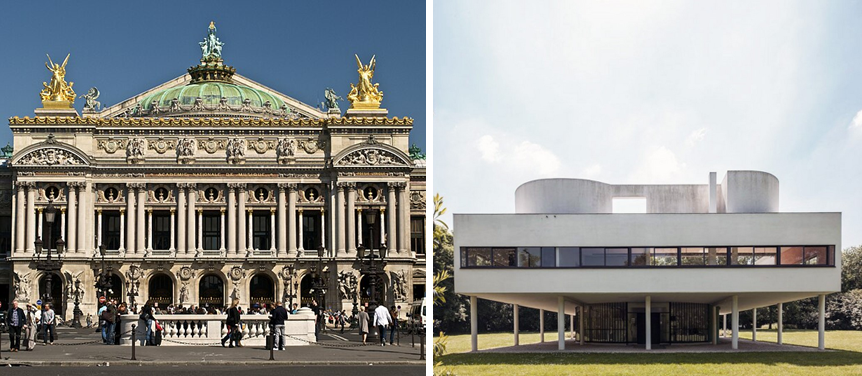
\includegraphics[width= \linewidth]{Images/NeoclassicismVsModernism}
          \caption{Neoclassic building "Paris Opera" 19th AC (left) vs Modernist house "Villa Savoye" 20th AC (right). From Complexity to simplicity. (\textit{Images edited from source: \cite{Stacbond2020}})}
          \label{fig:NeoclassicalvsModernism}
        \end{figure}

This architectural ethos adopted the maxim ``Form follows function'', emphasizing functionalism and characterized by a rejection of traditional ornament in favor of new forms of more subtles intricacies like the “aesthetics of machinery” that showcased architecture  enriched  with  only  the  beauty of its lines and the use of new-age materials such as steel, glass, and concrete\cite{Gage2015}.

%% add some extra references to the modernist section specially about the urban configuration 

The postmodernism style of the late 60's marks a radical return of ornament in form recognizing that even simplified modern elements serve as ornamentation focusing on the thought of freeing design element from oppresive modern constraints.

%%Figure neoclassicim vs modernism
     \begin{figure}[htb]
          \centering
          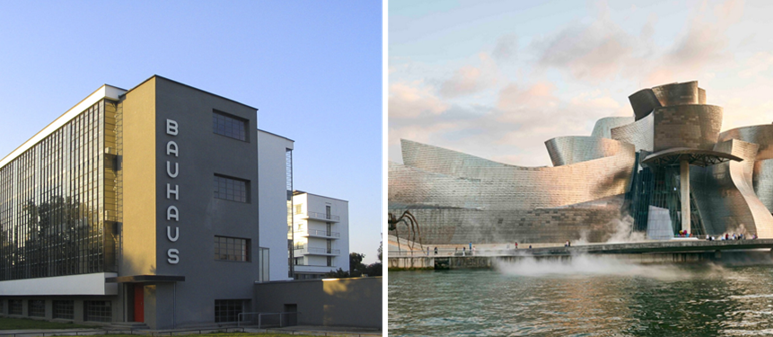
\includegraphics[width= \linewidth]{Images/modernism vs postmodernism}
          \caption{Modernist building "Bauhaus School" 20th AC (left) vs Postmodernist "Guggenheim museum" 1997 (right). From simplicity to Complexity. (\textit{Images edited from source: \cite{Arora2023}})}
          \label{fig:Modernismvspostmodernism}
        \end{figure}

The late 20th century embraced imagination and expression through architects like Frank Gehry, Zaha Hadid, and Rem Koolhaas.
Their constructions stood as monumental expressions of ornament, enabled by digital technologies.
Complex shapes and structures became reality, ranging from juxtaposed ornaments to transformative structural ornamentation.

However, due to their complexity, these structures remained exceptional, not integrated into the urban fabric.
The democratization of digital fabrication brings a paradigm shift, offering diverse cultures the means to express authenticity through complex designs.
This signals a contemporary era embracing complexity and ornament.

Amidst this historical exploration, it becomes evident that the architecture of the future is poised to harmonize ornamentation, functionality, and human comfort.
The trajectory points towards a style of complexity—a style that crafts a delicate equilibrium, resonating with the values of our time and the technological possibilities at our fingertips.

In this intricate interplay, architecture emerges as a tangible synthesis of human experience and creative expression, balancing ornament's aesthetic allure, the essential functionality of the built environment, and the crucial comfort of its inhabitants.

        ``If architecture is to exist in the 21st century, when attention is focused on the fast-paced worlds of technology, fashion, and entertainment, it must not recede into the background as mere functional equipment''\cite{Gage2015}.

%
\subsection{Cultural Significance of Facades and Ornament}
\label{subsec: FacadeandOrnament }
The resonance of Louis Sullivan's renowned phrase, ``Form follows function,`` throughout the Modernist movement of the 20th century and its continued influence on subsequent decades can be attributed to the pivotal role of a building's purpose and functions as the genesis and core of a project\cite{Hnin2022}.

This principle found its radicalization within the context of the times, partly due to a prevailing stance against ornamentation, often dismissed on moralistic grounds.
This sentiment deemed everything beyond function as secondary, exemplified by works like Adolf Loos' 1908 article ``Ornament and Crime,`` which advocated for functional design by condemning traditional ornamentation as superfluous\cite{Saglam2014}.

Even during this era when ornamentation was viewed unfavorably, prominent figures of the time, such as Le Corbusier, who publicly championed the functional ideology, would ingeniously devise methods to infuse their creations with a distinct form of ornamentation, albeit one rooted in materials' textures, structural elements, and inventive ways of articulating functionality.\cite{Saglam2014}.
In Venturi's opinion\cite{Venturi1972} 1960's ``Modern architecture uses expressive ornament and shuns explicit symbolic  ornament'' and all the simplistic facades are a type of ornament\cite{Saglam2014}.

          ``If architecture is to exist in the 21st century, when attention is focused on the fast-paced worlds of technology, fashion, and entertainment, it must not recede into the background as mere functional equipment''\cite{Gage2015}.

          According to Krier the mature city achieves balance with nature and with the people that it serves in its scale, size and integration of residential, commercial and civic functions.
          Krier argues that the reconstruction of a city is a moral imperative, a global project that it is at once cultural social economic and ecological. Time of video 1:06:29

We evidence this when observing the Romanesque classical style on the 10 th century found mostly in churches ith thick wall structures, followed by the breakthrough in load distribution during the Gothic style of the 12th to the 16th century which abandons the robustness to erect high buildings with complex great stained windows.
The Renaissance follows at the end of the Middle Ages and with it the return of the classical order with round arch and classical order columns that brings ornaments back to the interior in favour of more simplified exteriors.
In reaction to this style Baroque style surges with more dynamic forms , irregular shapes and exaggerated ornamentation in bold combinations.

%%%%
what initially motivates this research is the conscious realization that
Upon delving into the annals of influential architectural styles, a discernible pattern emerges—an oscillation between simplicity and complexity(see Figure\ref{fig:TimelineArchitecture}).
This recurrent cycle in architectural paradigms is not only reflective of the values ingrained in the societies they house, but also closely tied to pivotal technological advancements.
Consider, for instance, the transition from the Romanesque style of the 10th century to the Complex Gothic style 12th style, replaced by the revival of greek and roman ideals during the Renaissence style, followed by the complex opulent ornamentation of the Baroque style in the 16th century replaced by the neoclassical revival of the 18th century, heavily influenced by classical Greek and Palladian architecture\cite{Arora2023}.
This pattern repeats all the way to the 1920s and 30s, the intricate Art Deco will be replaced on the first half of the 20th century witnessed the emergence of Modern Architecture and rationalism emphasizing functionalism and minimalistic architecture




This shift encapsulates the quintessence of architectural evolution—an ever-changing interplay between simplicity and complexity, often steered by the confluence of societal values and technological breakthroughs.


Once again, we find ourselves at a pivotal juncture in history, as the emergence of computer-aided design converges with the industrialization of construction, ushering in a new paradigm in architectural design.
The 20th-century dominance of Rationalism, exemplified by figures like Le Corbusier, underscored an ethos of oversimplification and functionality.
Characterized by straightforward, symmetrical forms and concrete as the favored medium, this era yielded cities estranged from human-centric design.
Swift transportation took precedence, fracturing urban spaces that once defined vibrant societies\cite{Stacbond2020}.
Subsequently, industrial design asserted its dominance as the blueprint for future construction\cite{Economakis2023}, casting architecture in the mold of minimalism and mass-produced uniformity, forsaking the ornate allure and individuality of yesteryears.

\subsection{Object-Oriented Ontology}
\label{subsec:ObjectOrientedOntology}
% add the concept of Object-Oriented. Using these concepts as basis. I want to express that the mr experiment is based on the idea that architecture as a tool should be invisible and confortable while in use. But it should  create emotion when seen as part of the landscape as a form of art to recapture the humand oriented city .

Heideggers tool analysis states that as the tool is a tool it disappears in favor of some purpose he continues to explain that generally we don't notice equipment until it fails, like when An earthquake calls attention to the ground we walk or when a medical problem alerts us of the presence of organs that we have silently depended\cite{Harman2011}.
Harmans, Object-oriented ontology, borrows this concept to formulate its central claim that objects have hidden qualities and realities, and they withdraw from our understanding.\cite{Gage2015}
he idea that we live our lives on a layer of invisible equipment has significant ramifications for architecture, a discipline that produces the equipment on and in which we exist.\cite{Gage2015}
